\section{Asymmetric cryptosystems}

Desirable features include the ability to establish a short secret agreement over a public channel, send messages confidentially over an authenticated public channel without sharing secrets with recipients, and authenticate actual data.

The solution lies in asymmetric cryptosystems, which revolutionized cryptography. Before 1976, methods relied on human carriers or physical signatures. 
Then, innovations such as the Diffie-Hellman key agreement in 1976, public key encryption in 1977, and the introduction of digital signatures in the same year paved the way for modern cryptographic solutions.

\paragraph*{Note}
Until now, the most effective attack method has been enumerating the secret parameter. 
This approach suffices for modern block ciphers, with the best attack requiring approximately $\mathcal{O}(2^\lambda)$ operations.
However, asymmetric cryptosystems depend on complex computational problems, where brute-forcing the secret parameter is not the optimal strategy. 
For instance, factoring a number of $\lambda$ bits demands computational effort approximately $\mathcal{O}\left(e^{k(\lambda)^\frac{1}{3} \cdot \log(\lambda)^\frac{2}{3}}\right)$.
It's crucial to note that comparing the sizes of security parameters rather than their actual complexities can lead to misleading conclusions.

\subsection{Diffie-Hellman key agreement}
The objective of the Diffie-Hellman key agreement protocol is to enable two parties to securely share a secret value using only public messages.
Assuming an attacker model where interception of communications is possible, but tampering is not, and relying on the Computational Diffie-Hellman (CDH) assumption, the protocol operates under the following principle:
\begin{itemize}
    \item Let $\left(\mathsf{G},\cdot\right)\equiv \left\langle g \right\rangle $ represent a finite cyclic group, with two randomly sampled numbers $a$ and $b$ from the set $\left\{ 0,\dots,\left\lvert \mathsf{G} \right\rvert  \right\}$, where the length of a ($\lambda = \text{len}(a)$) is approximately logarithmic to the size of $\mathsf{G}$.
    \item Given $g^a$, $g^b$, the computational complexity of finding $g^{ab}$ is significantly greater than polynomial in the logarithm of the size of $\mathsf{G}$.
    \item The most effective current attack strategy involves solving either for $b$ or $a$, known as the discrete logarithm problem.
\end{itemize}
\begin{example}
    Let's consider two users, A and B:
    \begin{itemize}
        \item User A selects a random number $a$  from the set  $\left\{ 0,\dots,\left\lvert \mathsf{G} \right\rvert  \right\}$ and sends $g^a$ to user B. 
        \item User B selects a random number $b$  from the set  $\left\{ 0,\dots,\left\lvert \mathsf{G} \right\rvert  \right\}$ and sends $g^b$ to user A. 
        \item User A receives $g^b$ from user B and computes $\left(g^b\right)^a$. 
        \item User B receives $g^a$ from user A and computes $\left(g^a\right)^b$. 
    \end{itemize}
    Because the finite cyclic group $\left(\mathsf{G},\cdot\right)$ is commutative, we can observe that $\left(g^b\right)^a=\left(g^a\right)^b$. 
\end{example}
In practical implementations, a subgroup $\left(\mathbb{Z}_N^\ast,\cdot\right)$  is chosen from $\left(\mathsf{G},\cdot\right)$, where $\mathbb{Z}_N^\ast$ denotes the set of integers modulo $n$ 

In this scenario, breaking the computational Diffie-Hellman assumption requires a minimum of:
\[\min \left( O\left( e^{k\log(n)^{\frac{1}{3}}\cdot\log(\log(n))^{\frac{2}{3}}}\right), O\left(2^\frac{\lambda}{2}\right)\right)\]
Alternatively, when utilizing elliptic curve points with dedicated addition, breaking the computational Diffie-Hellman assumption takes $O\left(2^\frac{\lambda}{2}\right)$ time. 

\subsection{Public key encryption}
In public key encryption, distinct keys are utilized for decryption and encryption purposes. 
It is computationally challenging to accomplish two tasks: decrypting a ciphertext without access to the private key and computing the private key solely from the public key.
\begin{figure}[H]
    \centering
    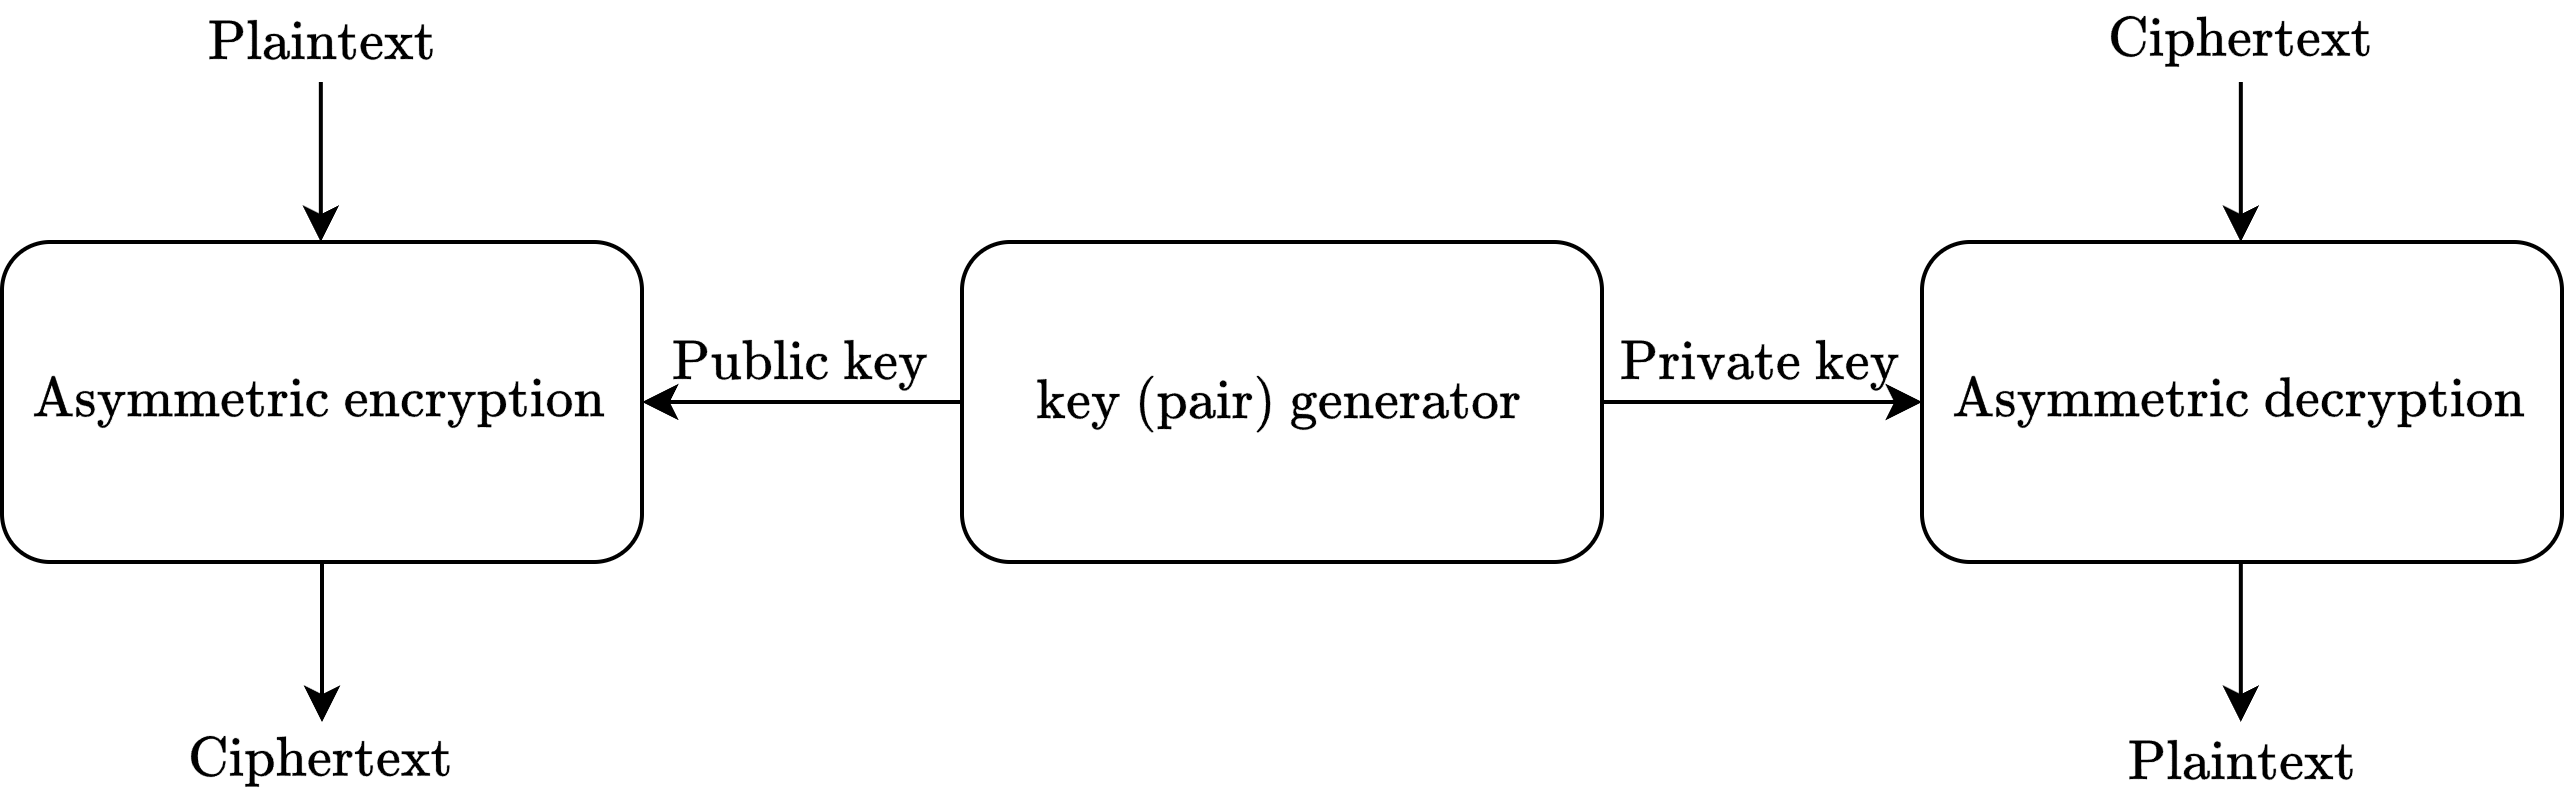
\includegraphics[width=0.75\linewidth]{images/ke.png}
    \caption{Key encryption}
\end{figure}

\paragraph*{Algorithm}
Rivest, Shamir, Adleman (RSA) is a groundbreaking encryption algorithm introduced in 1977. 
It supports message and key sizes ranging from 2048 to 4096 bits, ensuring robust security against modern computational threats.
Originally patented, RSA's intellectual property rights have since expired, fostering widespread adoption and further development within the cryptographic community.
One notable advantage of RSA is its capability to encrypt messages without expanding ciphertext, ensuring efficient transmission and storage of encrypted data.
Additionally, RSA encryption with a fixed key exhibits pseudorandom permutation (PRP) properties, enhancing its versatility and applicability in various cryptographic scenarios.

The ElGamal encryption scheme, conceived in 1985, offers a versatile cryptographic solution characterized by its flexibility and patent-free nature.
ElGamal encryption accommodates keys spanning either the k-bit range or hundreds of bits, contingent upon the chosen variant, allowing for tailored security configurations to suit various applications.
Free from patent encumbrances, the ElGamal scheme has gained traction as a viable alternative to RSA, particularly in scenarios where patent restrictions were a consideration.
A distinctive attribute of ElGamal encryption is its ciphertext, which typically spans twice the size of the plaintext. 
Despite this expansion, its widespread adoption attests to its effectiveness in safeguarding sensitive data and communications.

\paragraph*{Usage}
Key encapsulation is a cryptographic technique used to securely transmit secret keys between parties over an insecure communication channel. 
In this method, the secret key is encapsulated or wrapped within another encryption layer using a public key algorithm. 
The recipient, possessing the corresponding private key, can then decrypt and extract the encapsulated key.
\begin{example}
    Let's consider a scenario where there exists a public channel between users A and B, and the attacker can only observe but not alter the communication.
    Subsequently, user B randomly selects a bitstring $s$ from the set $\left(k_{pri},k_{pub}\right)$ encrypts it using $k_{pub}$, and forwards the resulting ciphertext to user A. 
    User A, possessing the corresponding private key $k_{pri}$, decrypts the ciphertext and retrieves the bitstring $s$. 

    The process is then repeated with the roles of users A and B swapped. 
    Consequently, both users obtain separate secrets. 
    Although user B alone determines the value of the shared secret $s$, combining the two secrets derived from the exchanged messages yields analogous security guarantees to those of a conventional key agreement protocol.
\end{example}
Using an asymmetric cryptosystem, user B encrypts a message for user A without the requirement of pre-shared secrets. 
Theoretically, user B and user A could rely solely on an asymmetric cryptosystem for their communication needs. 
However, in practice, this method would prove highly inefficient.
Asymmetric cryptosystems operate significantly slower compared to their symmetric counterparts, with performance degradation ranging from 10 to 1000 times.

\paragraph*{Modern encryption}
Hybrid encryption schemes represent a strategic blend of asymmetric and symmetric cryptography techniques.
In this approach, asymmetric algorithms are utilized for key transport or agreement, facilitating secure key exchange between parties. Meanwhile, symmetric algorithms are employed to encrypt the bulk of the data, ensuring efficient and swift encryption of large volumes of information. 
This concept serves as the cornerstone for all contemporary secure transport protocols, embodying a harmonious integration of both cryptographic methodologies to deliver robust and effective encryption for secure communication.
\begin{figure}[H]
    \centering
    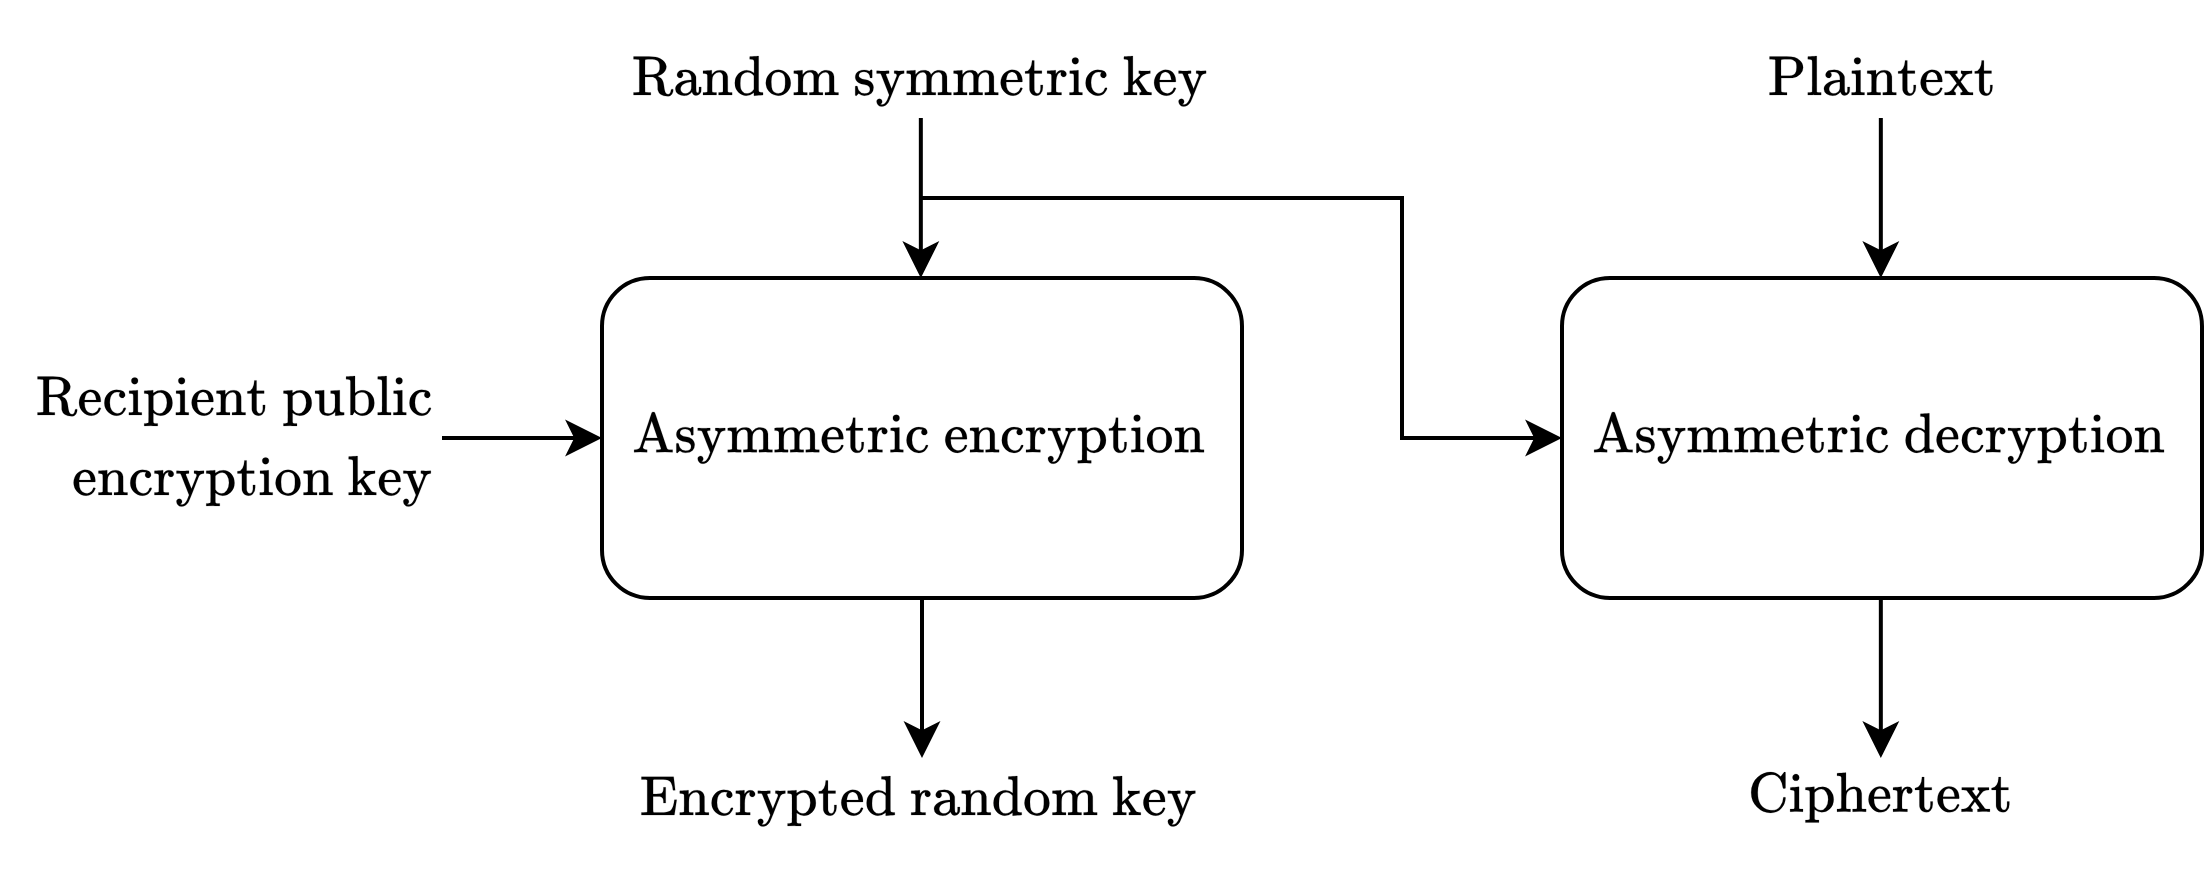
\includegraphics[width=0.75\linewidth]{images/menc.png}
    \caption{Modern encryption}
\end{figure}

\subsection{Digital signatures}
Authenticating data serves as a crucial aspect in the establishment of secure hybrid encryption schemes. 
It ensures that the public key utilized by the sender corresponds accurately to the intended recipient. 
Additionally, the ability to verify the authenticity of data without relying on a pre-shared secret is highly desirable.
Digital signatures play a pivotal role in achieving data authentication objectives:
\begin{itemize}
    \item They offer robust evidence linking data to a specific user, enhancing data integrity.
    \item Verification of digital signatures does not necessitate a shared secret, simplifying the authentication process.
    \item Properly generated digital signatures cannot be repudiated by the user, ensuring accountability.
    \item Asymmetric cryptographic algorithms underpin digital signatures, providing a solid foundation for their security.
    \item It has been formally demonstrated that achieving non-repudiation without digital signatures is impractical, reinforcing their indispensable role in data authentication.
\end{itemize}
\begin{figure}[H]
    \centering
    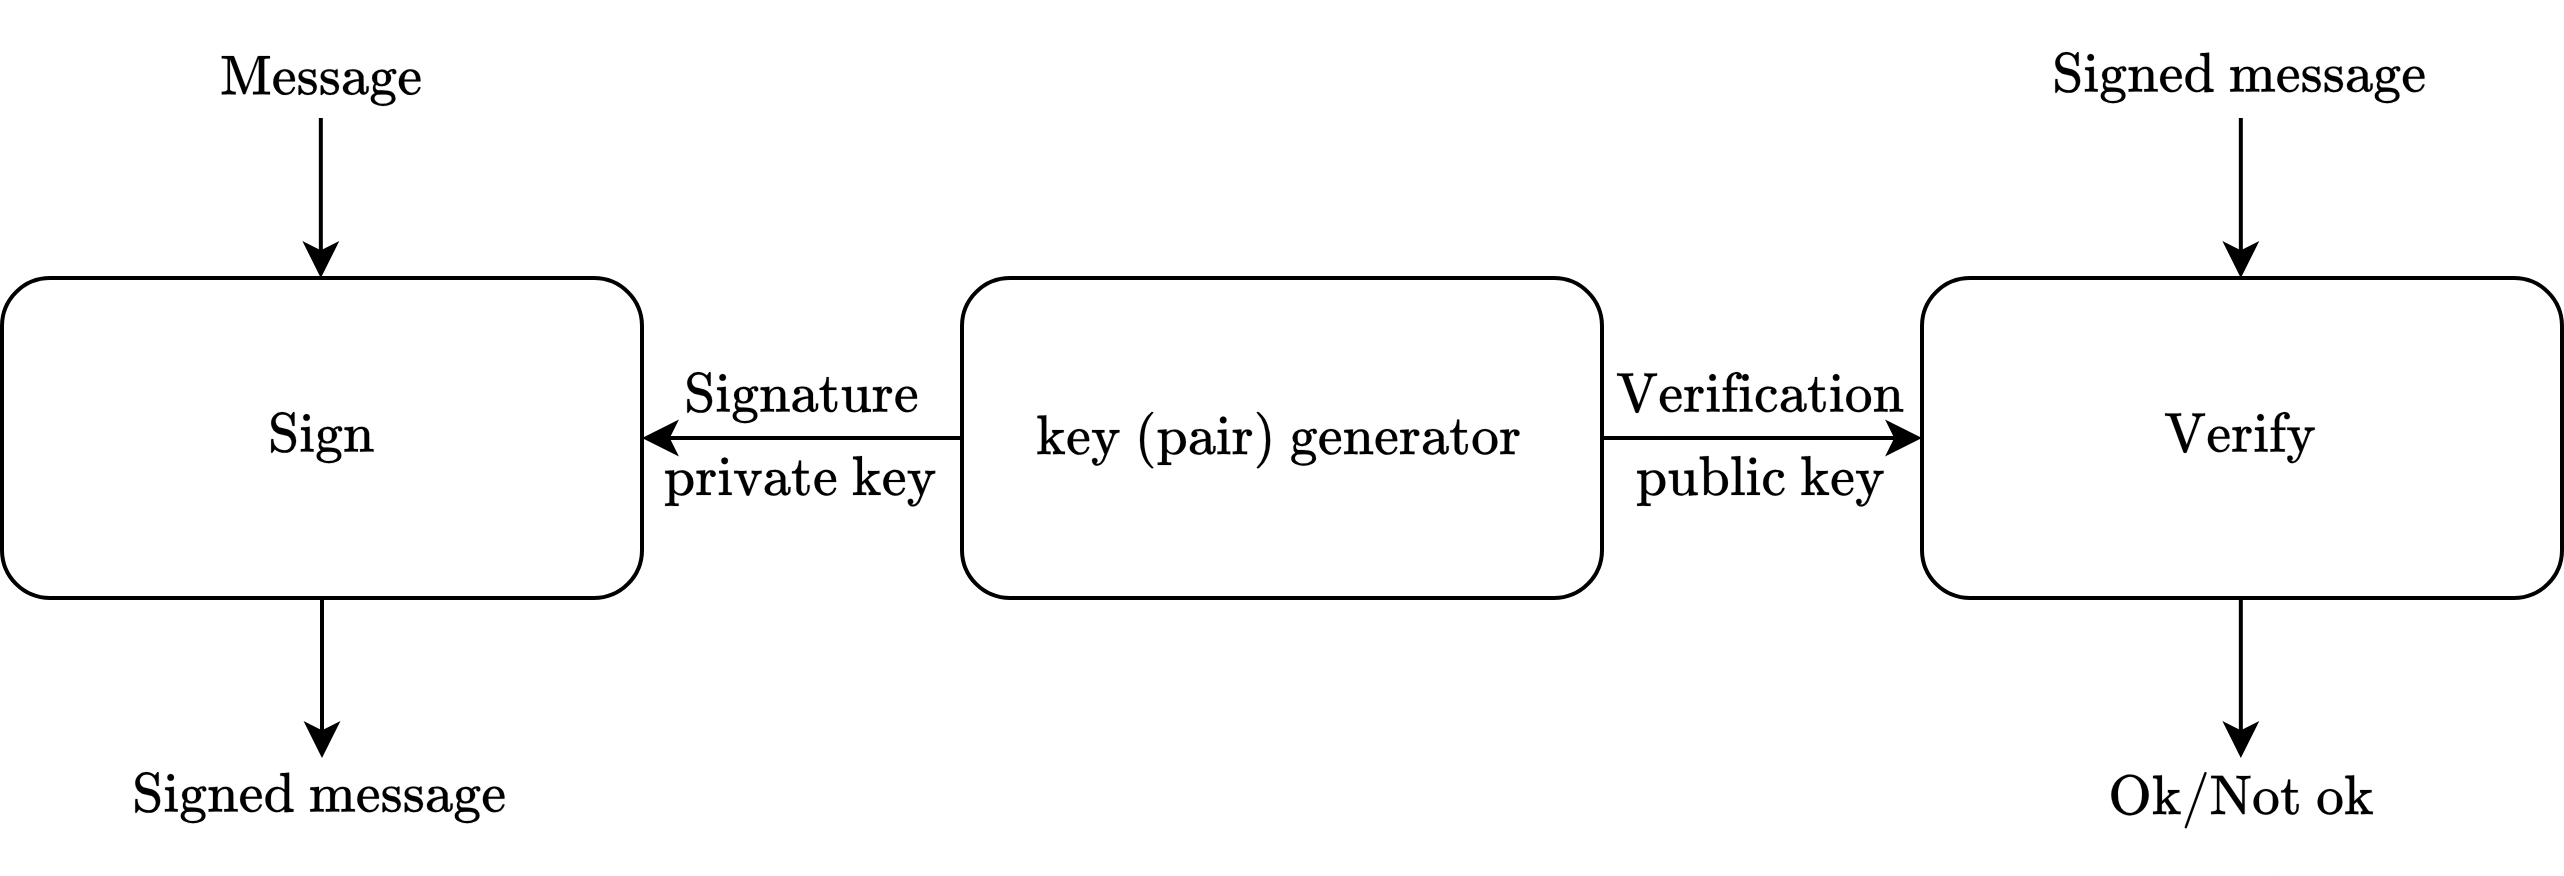
\includegraphics[width=0.75\linewidth]{images/aut.png}
    \caption{Digital signature}
\end{figure}
The computational challenges inherent in digital signatures encompass several key aspects:
\begin{itemize}
    \item Signing a message without possessing the signature key, which includes attempting to splice signatures from unrelated messages.
    \item Computing the signature key when provided only with the verification key.
    \item Attempting to derive the signature key solely from signed messages, without access to additional information.
\end{itemize}

\paragraph*{Algorithms}
In 1977, Rivest, Shamir, and Adleman (RSA) introduced a groundbreaking cryptographic method. 
This method employs a singular hard-to-invert function to craft both an asymmetric encryption scheme and a signature, with distinct message processing for each. 
Notably, the process of signing is significantly slower than verification, roughly around 300 times slower. 
This innovative approach has been standardized in NIST DSS (FIPS-184-4), underscoring its widespread adoption and importance in modern cryptographic practices.

The Digital Signature Standard (DSA) draws its foundations from adjustments made to signature schemes initially proposed by Schnorr and ElGamal. 
It, too, has been formalized in NIST DSS (FIPS-184-4), reflecting its establishment as a recognized cryptographic protocol. 
Notably, in DSA, the processes of signature creation and verification unfold at comparable speeds, distinguishing it from some other cryptographic methods.

\paragraph*{Usages}
Digital signatures serve various purposes:
\begin{itemize}
    \item Authenticating digital documents: in order to enhance efficiency, digital signatures frequently entail signing the hash of a document rather than the document itself. 
        However, the assurance of the signature's reliability relies on the robustness of both the signature and hash algorithms.
    \item Authenticating users: digital signatures present an alternative approach to user authentication, serving as a viable replacement for traditional password-based logins. 
        During this procedure, the server retains the user's public verification key, typically acquired during the account creation phase. 
        Upon authentication requests, the server initiates the client to sign a lengthy, randomly generated bitstring, referred to as a challenge. 
        Successful verification of the challenge signature by the client serves as compelling evidence of identity to the server.
\end{itemize}